
\chapter{Conexión desde el navegador local}
\section{Enunciado}
8. Conexión desde el navegador local. Firefox debe acceder sin mostrar ningún error. No permitir la conexión si aparecen errores del tipo ``entiendo los problemas...''.
\section{Resolución}
Se realizan pruebas con Firefox, donde deberá accederse de forma transparente, es decir, sin mostrar ningún error y 
sin generar avisos con la opción de "\textit{Entiendo los riesgos}". Para ello, además de añadir el certificado raíz de la CA 
de la asignatura a la lista de autoridades de confianza del sistema, se ha añadido el certificado raíz de la CA de la asignatura a 
la lista de autoridades de confianza del navegador Firefox.
\begin{figure}
    \centering
    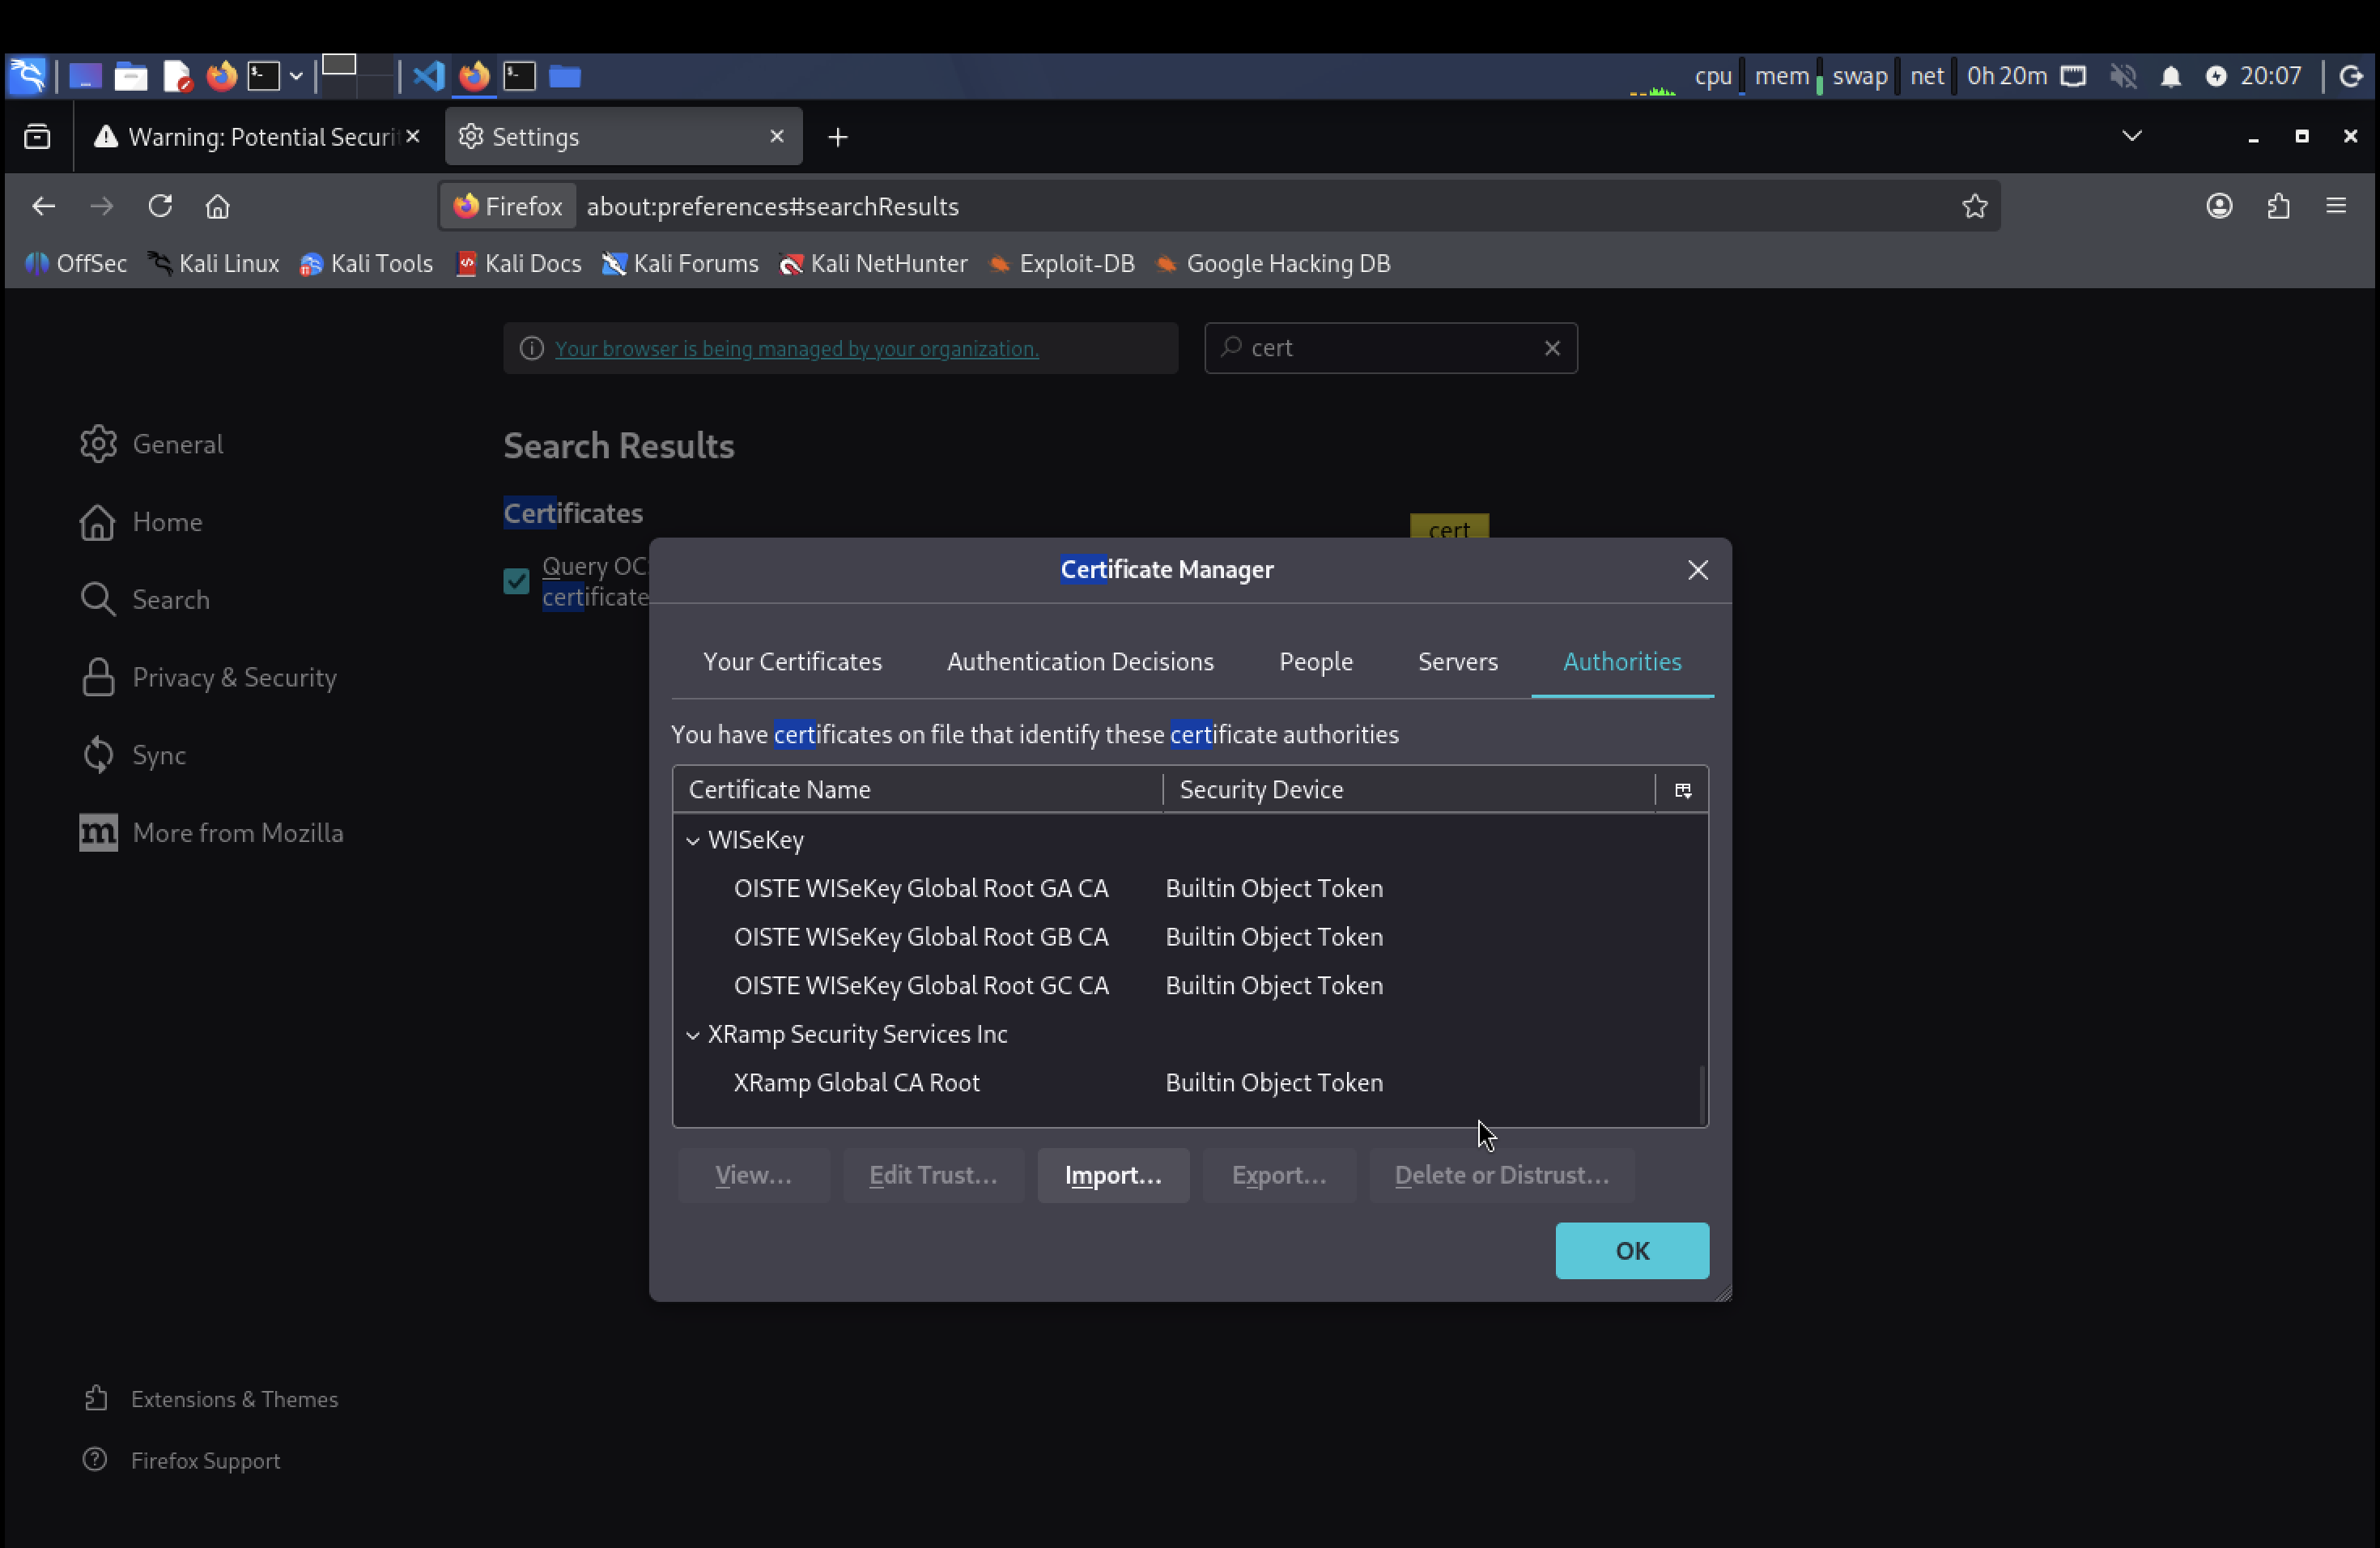
\includegraphics[width=0.8\textwidth]{Imagenes/18.png}
    \caption{Añadir el certificado raíz de la CA de la asignatura a la lista de autoridades de confianza del navegador Firefox.}
\end{figure}
\begin{figure}
    \centering
    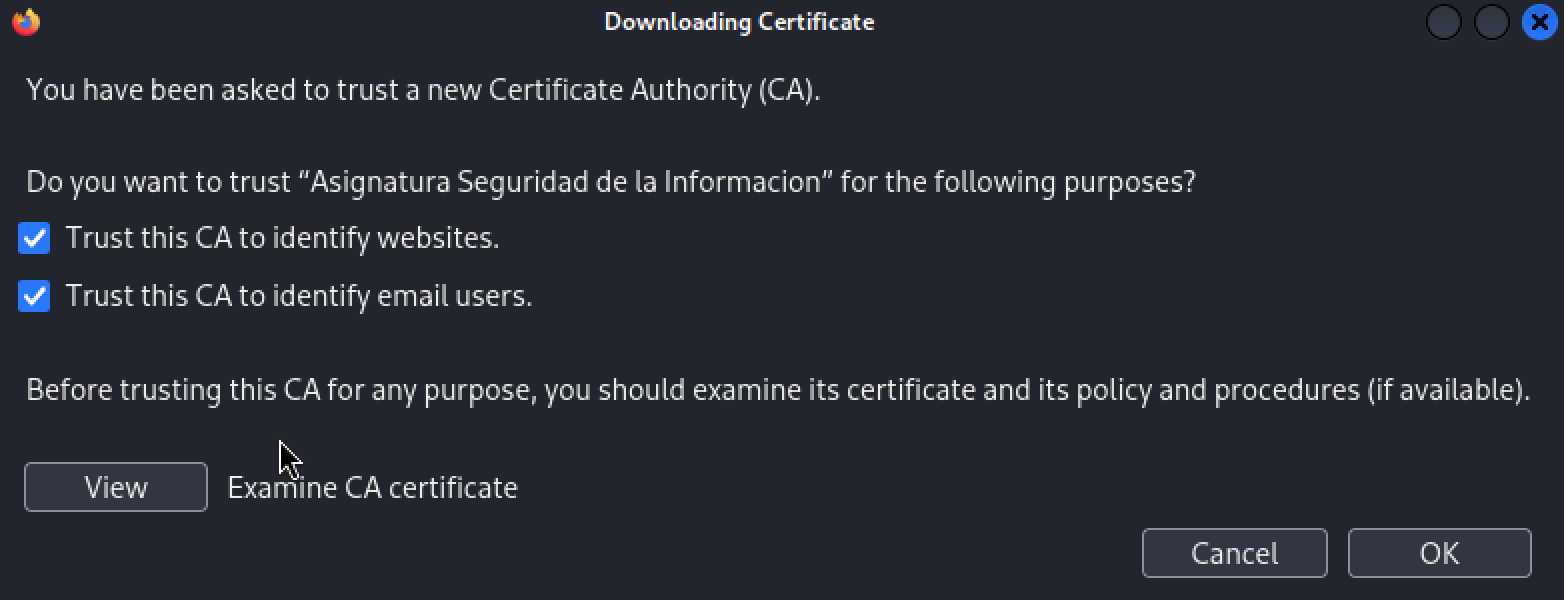
\includegraphics[width=0.8\textwidth]{Imagenes/19.png}
    \caption{Añadir el certificado raíz de la CA de la asignatura a la lista de autoridades de confianza del navegador Firefox.}
\end{figure}
\begin{figure}
    \centering
    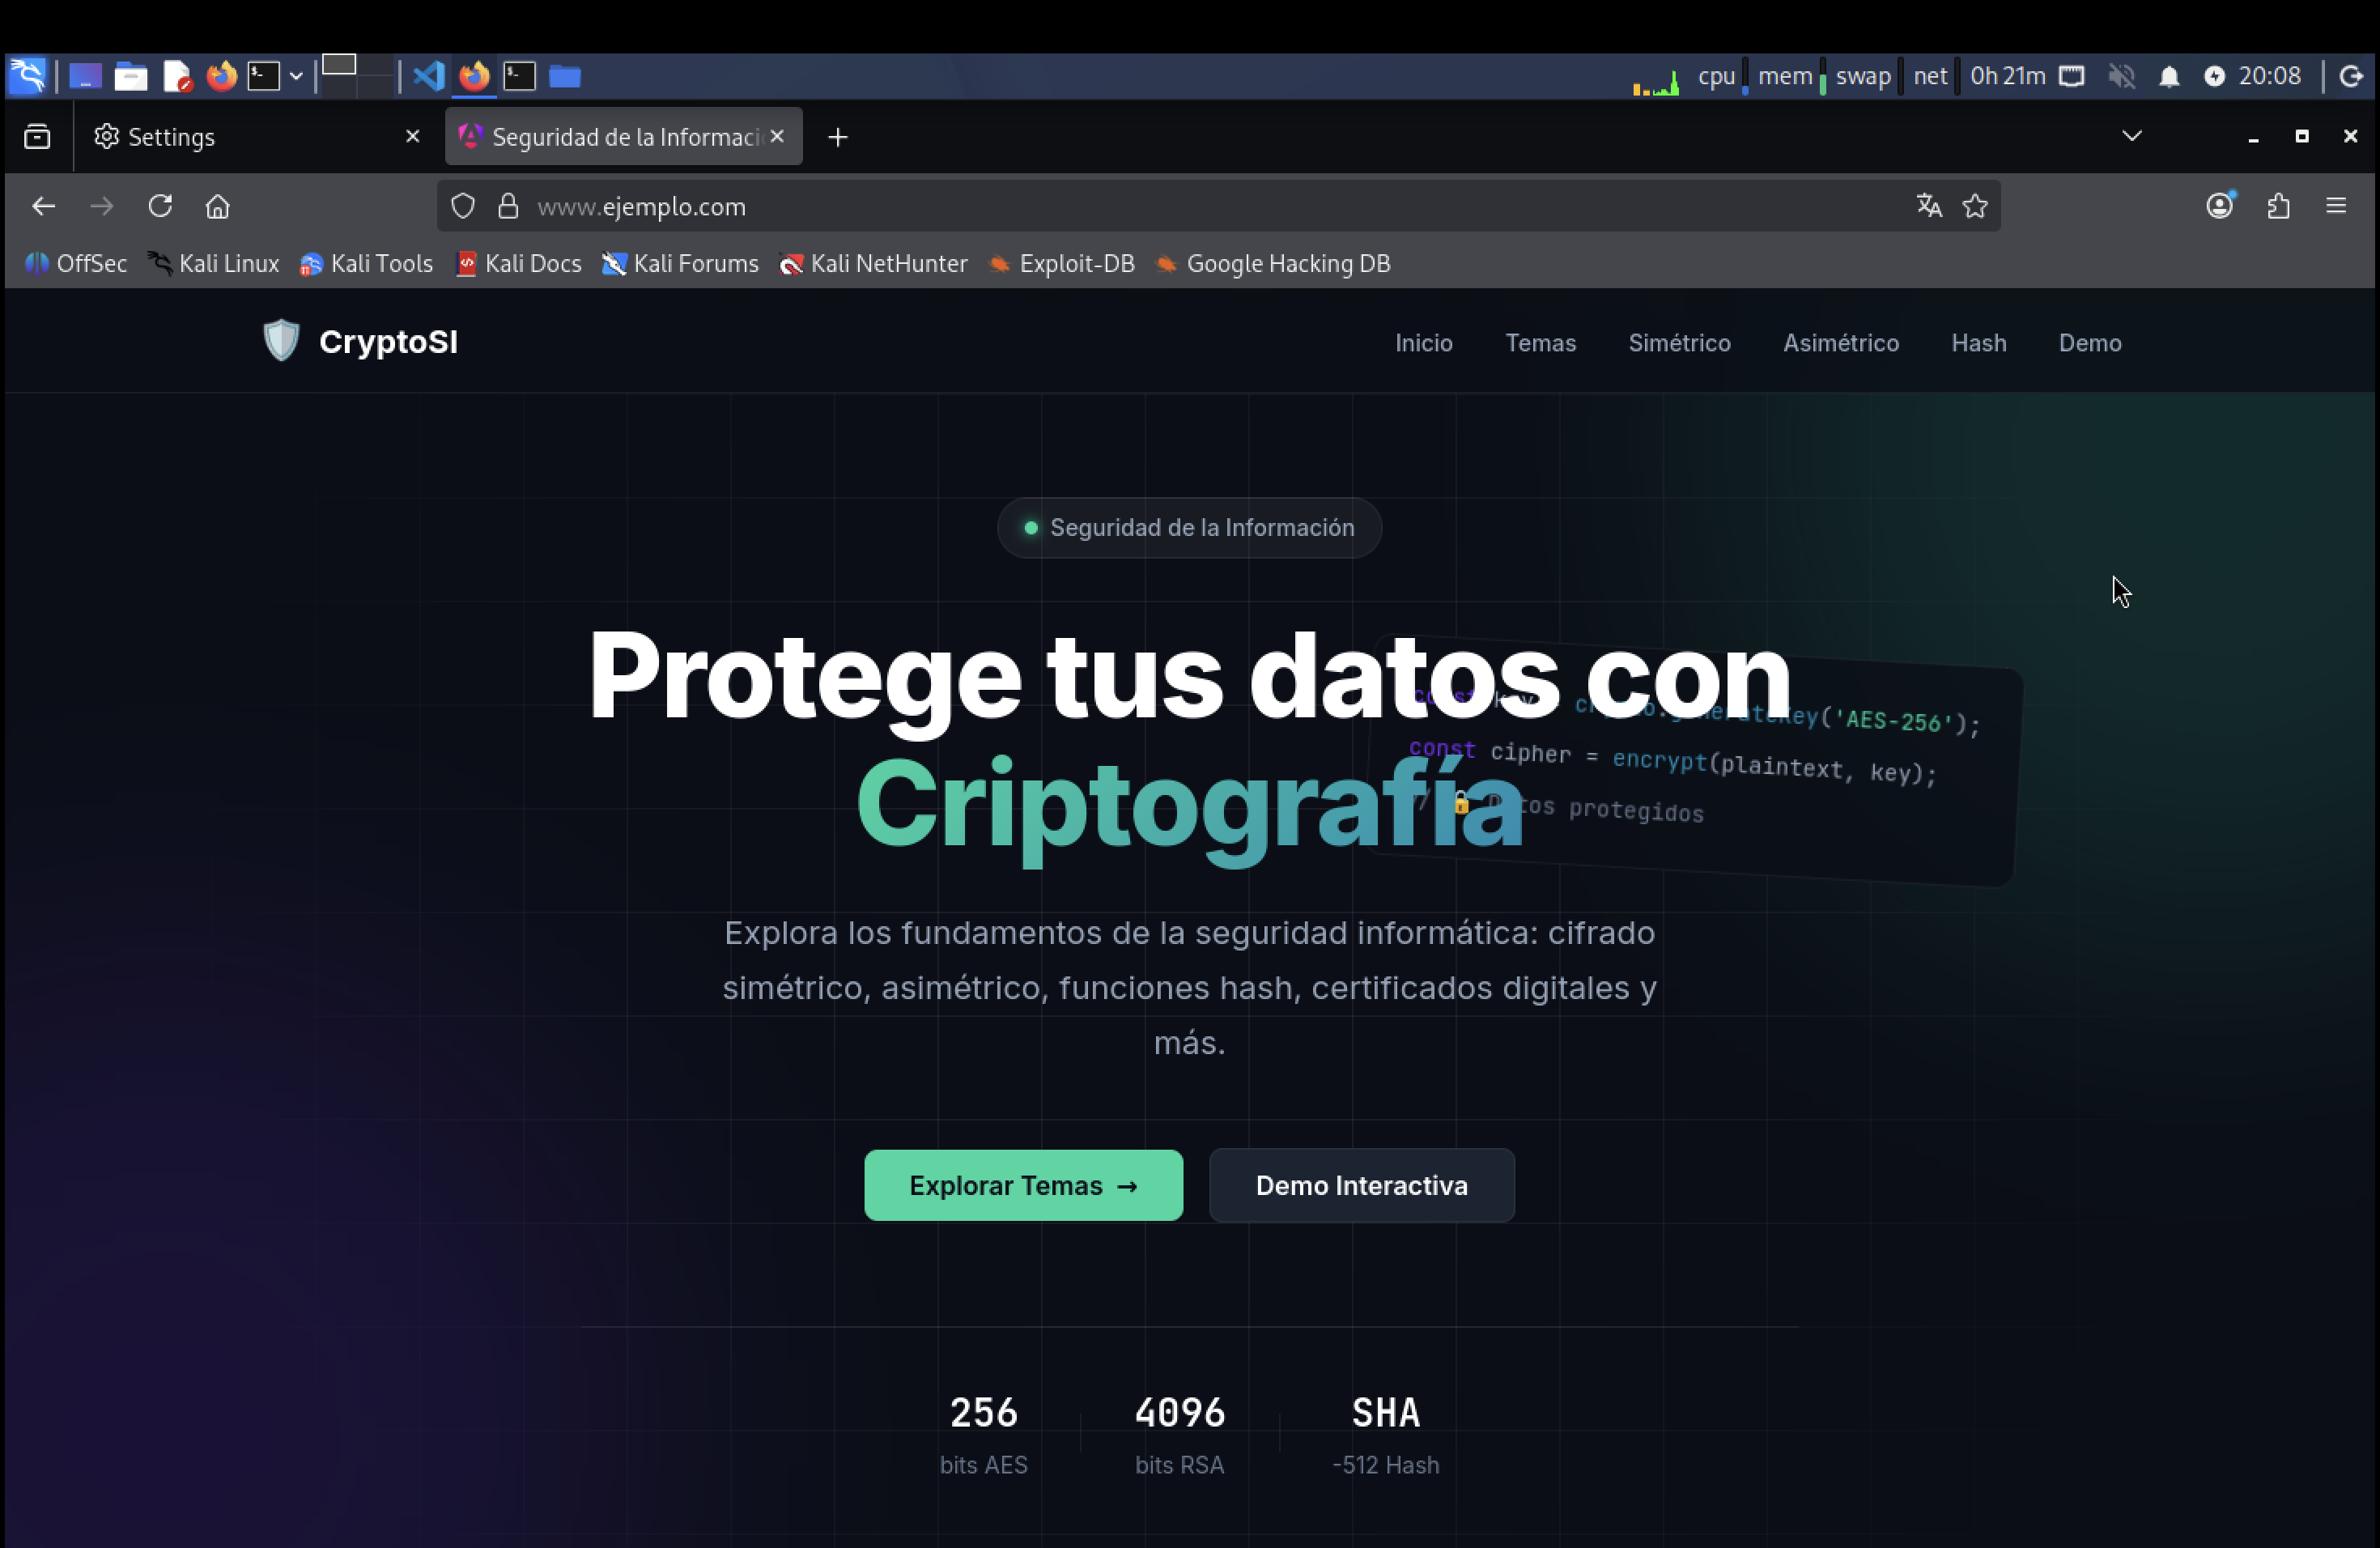
\includegraphics[width=0.8\textwidth]{Imagenes/20.png}
    \caption{Acceso al sitio web desde Firefox.}
\end{figure}
